\documentclass[../main.tex]{subfiles}

\begin{document}

\begin{figure}[bh]
    \centering
    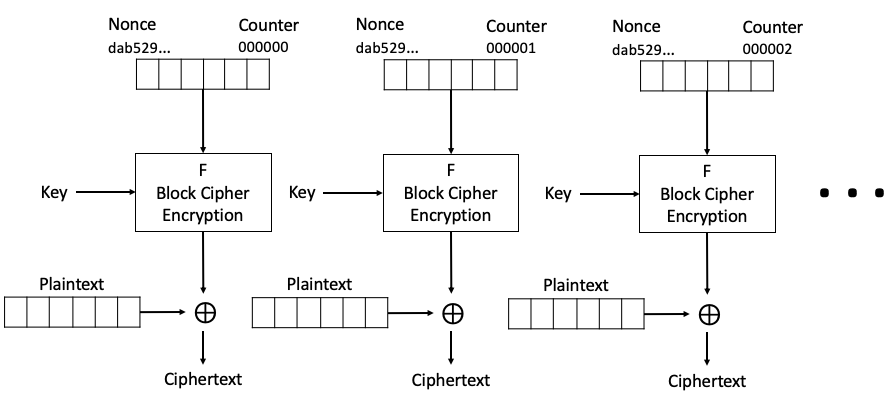
\includegraphics[width=\textwidth]{../../images/appendix/aes_ctr}
    
    \caption{AES CTR encryption}
    \label{appendix:figure:aes_ctr}
\end{figure}

\par From the above Figure \ref{appendix:figure:aes_ctr}, the scheme is mainly build on a complex block cipher F. And we have the following equation:
\begin{equation}
    C = P \oplus F(Key, IV)
\end{equation}
\par In this situation, if a user reuses the same Key/IV pair, we would obtain the following ciphertexts:
\begin{equation}
    \begin{split}
        C_1 = P_1 \oplus F(Key, IV)\\
        C_2 = P_2 \oplus F(Key, IV)
    \end{split}
\end{equation}
\par This implies that an attacker can then compute with ease:
\begin{equation}
    C_1 \oplus C_2 = P_1 \oplus P_2
\end{equation}
\par And derive the values of the two plaintexts xored together without even knowing neither the key or the IV.

\end{document}